\section{Tomcat : conteneur de servlet Java EE}
%Nicolas
\subsection{Presentation}
\frame{\frametitle{Présentation Tomcat}
  \begin{itemize}
    \item Projet open-source de la fondation Apache
    \item Un serveur d'applications Java
    \begin{itemize}
      \item Java Servlet
      \item JavaServer Pages
    \end{itemize}
    \item Souvent utilisé avec un serveur web
  \end{itemize}
  }
\frame{\frametitle{Présentation Tomcat}
		\framesubtitle{Serveur d'application}
  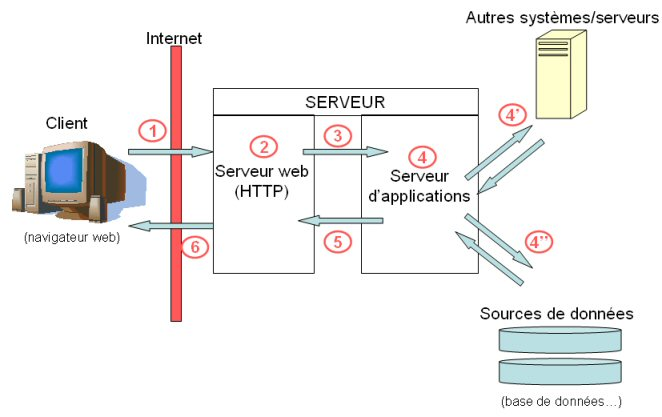
\includegraphics[scale=0.5]{Images/serveurapp.png}
}

\frame{\frametitle{Configuration Tomcat}

		\framesubtitle{Arborescence}
		Répertoire d'installation : CATALINA\_HOME
\begin{itemize} 
    \item \textbf{bin/} exécutables de Tomcat(démarrage du serveur)
    \item \textbf{common/} classes et librairies partagées par les applications web
    \item \textbf{conf/}
    \item \textbf{Logs/}
    \item \textbf{server/} contient les applications web du serveur en lui-même
    \item \textbf{shared/} contient les classes et librairies partagées par toutes les applications web hébergées sur le serveur
    \item \textbf{temp/}
    \item \textbf{webapps/} contient les applications web
    \item \textbf{work/} contient les JSP compilées
\end{itemize} 
}


\frame[containsverbatim]{\frametitle{Configuration Tomcat}
		\framesubtitle{Server.xml}
		Eléments Engine et Host
		\begin{itemize} 
   		\item \textbf{Elément Engine} : modélise le moteur de servlet, contient un ou plusieurs
hosts
    	\item \textbf{Elément Host} hôte virtuel (doit être associé à l'adresse IP de cen serveur)
		\end{itemize}

		\begin{lstlisting}
<Engine name="Catalina">
<Host name="localhost" appBase="webapps"
unpackWARs="true" autoDeploy="true">
<!-- contenu de l'élément Host -->
</Host>
</Engine>
		\end{lstlisting}
}
